In the preceding section, we described how an implicit surface representation can be used to create an atlas of local charts. We also mentioned the existence of an algorithm for creating an atlas by using an RRT path planning algorithm. We now continue with a description of how to bring these two elements together into what we term the GPAtlasRRT strategy. 

\begin{figure*}[t]
    \centering
    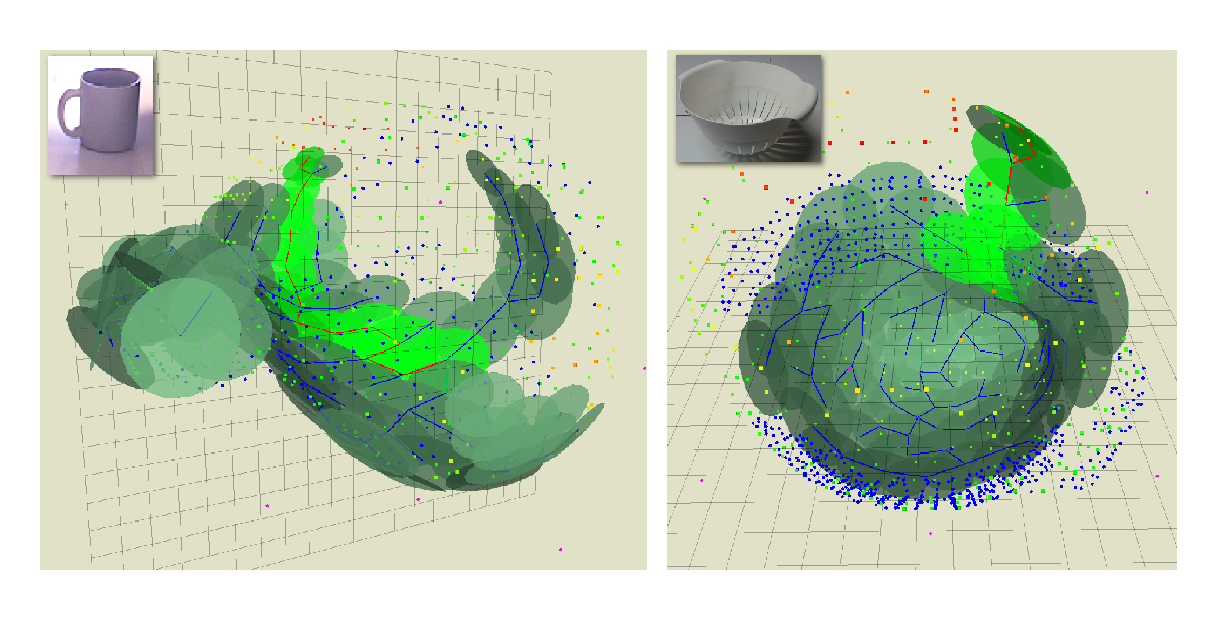
\includegraphics[width=0.95\linewidth]{twoAtlas.eps}
    \caption{The AtlasRRT expanding across the implicit surfaces of a mug (left) and a colander (right). The RRT used to create the atlas is marked in blue. The selected sequence of charts is highlighted in light green, and the associated path is marked in red (it is slightly obscured in the right panel). The robot tries to touch the object at the centre of each chart in the sequence. Both objects are viewed from above.}
    \label{fig:GPAtlasRRTtwo}
\end{figure*}

The method starts from an incomplete observation of the object surface with a depth camera. To this end, we assume there is a way to segment the object from the background scene\footnote{We provide technical details of our approach in Subsection~\ref{sec:real}}. 
%However, there might be no information at all, in which case the probe must naively move towards the palm of the gripper holding the object to obtain a first initial observation. 
%The paucity of the initial shape estimate will increase the time to converge to an accurate shape. 
The initial observations $\mathcal{S}^0$ are used to infer the implicit surface model, $\mathcal{GP}$ and to start to build the atlas. Algorithm \ref{alg:strategy} describes how the atlas is built so as to generate candidate points for tactile exploration which will improve the implicit surface model, $\mathcal{GP}$, so as to a predefined maximum variance, $\mathbb{V}_{\max}$. 

The first step is \textsc{selectSurfacePoint} (line \ref{init}) which randomly obtains a point $\mathbf{x}_i \in \mathcal{X}^0$ on which the first chart will be centred, invoking the \textsc{createChart} function (line \ref{create_chart}). The generated data structure for a chart contains: its centre, $\mathbf{x}_i$; the orthonormal tangent basis provided by (\ref{eq:tangent_basis}) $\boldsymbol{\Phi}_i$; $\nabla f(\mathbf{x})$ is equivalent to (\ref{eq:gradient_f}); its radius is $\rho_i$; and $\mathcal{U}_i$ is a set of points in the tangent space. Two things differentiate this from the original AtlasRRT algorithm. First, the size of a chart, also termed its validity region, is inversely proportional to the variance at the chart centre, namely,
\begin{equation}
\rho_i \propto \mathbb{V}[f(\mathbf{x}_i)]^{-1}.
\end{equation}
$\rho_i$ is thus actually the radius of a ball centred at $\mathbf{x}_i$, whose intersection with the tangent space yields the disk-shaped \emph{chart}. The motivation behind this choice is that the more certain a point is to be on the surface, the larger the region of its chart on the predicted shape, whereas if more uncertainty is associated with the centre, smaller exploratory steps will be preferred. Second, a number of points proportional to the size of the chart are sampled from a random uniform density on an annulus of the disk with internal and external radius $0.8\rho$ and $\rho$ respectively. The cardinality of this point-set in the tangent space is proportional to its size, namely,
\begin{equation}
\#\mathcal{U}_i \propto \rho_i.
\end{equation}
This implies that the larger the chart the more samples are needed to obtain a good quantization of it.\footnote{Another advantage of working with a normalized and offset-free set, as mentioned in Subsection \ref{sec:gpis}, is that the parameters that make the latter two expressions equal are tuned once, and remain fixed.}

\begin{algorithm}[t]
    \textbf{$\mathcal{P} \leftarrow$ \textsc{GPAtlasRRT}}($\mathcal{M}$, $\mathbb{V}_{\max}$)\\ %functionname
\LinesNumbered
\DontPrintSemicolon
\SetAlgoVlined \SetKwInOut{Input}{input} \SetKwInOut{Output}{output}
\Input{A Gaussian Process model, $\mathcal{M}$ and the set of parameters $\Omega$, defining criteria to decide how to start, extend and end the exploration.}
\Output{The best next action, $\mathcal{P}$, in the form of a path, if any, or $\varnothing$ otherwise.}
$\mathbf{x_i} \leftarrow$ \textsc{selectSurfacePoint}($\mathcal{GP}$) \label{init} \\ 
$\mathcal{C}_{i} \leftarrow$\textsc{createChart}($\mathbf{x}_i$, $\mathcal{GP}$) \label{create_chart} \\
% $\mathcal{A}, \mathcal{T}, \mathbf{x}_{c,i} \leftarrow$\textsc{init}($\mathcal{M}$, $\Omega$) \\
$\mathcal{A} \leftarrow$ \textsc{addChart}($\mathcal{C}_i$) \label{add_chart} \\
  \label{is_expandable} \While{ \textsc{isExpandable}($\mathcal{A}$) }
  {
    $\mathcal{C}_j \leftarrow$\textsc{selectChart}($\mathcal{A}$) \label{select_chart} \\
    $\mathbf{x}_k \leftarrow$\textsc{expandChart}($\mathcal{C}_j$, $\mathcal{GP}$) \label{expand_chart} \\
    $\mathcal{C}_k \leftarrow$ \textsc{createChart}($\mathbf{x}_k$, $\mathcal{GP}$) \label{create_new_chart} \\
    $\mathcal{A} \leftarrow$\textsc{addChart}($\mathcal{A}$, $\mathcal{C}_k$) \label{add_new_chart} \\
    \label{ending} \If{ $\mathbb{V}[f(\mathbf{x}_k)]  > \mathbb{V}_{\max}$ }
    {
      $\mathcal{P} \leftarrow$ \textsc{getPath}($\mathcal{C}_i$, $\mathcal{C}_k$) \label{compute_path} \\
      \Return $\mathcal{P}$ \label{return_path} \\
    }
    % \textsc{connect}($\mathcal{T}$, $\mathcal{C}_{k}$, $\mathcal{C}_{j}$) \\
    %$\mathcal{C}_{i} = \mathcal{C}_{k}$ \\
  }
  %\eIf {\textsc{solution}($\mathcal{C}_{i}$)}
  %{\Return $\mathcal{P} \leftarrow$\textsc{path}($\mathcal{C}_{i}, \mathcal{T}$)}
  \Return $\varnothing$ \label{no_candidate}
  \caption{GPAtlasRRT} \label{alg:strategy}
\end{algorithm}

The first chart is the root node of an exploration tree (line \ref{add_chart}). The question whether an atlas \textsc{isExpandable} or not (line 4) is answered by checking whether there is at least one chart $i$ with $\#\mathcal{U}_i \neq 0$. If the predicted surface is completely covered with charts the while condition will fail and the algorithm terminates (line \ref{no_candidate}), otherwise it loops. The first step selects a chart to expand (\textsc{selectChart}, line \ref{select_chart}) from those charts $i$ with a non-empty point-set $\mathcal{U}_i \neq \emptyset$. Tree expansion is either depth-first (selecting the most recently created chart), with probability $p = 0.4$, or a randomised sample (across other charts), with probability $1-p$. In the first iteration, $\mathcal{C}_i$ is the only chart, and thus guaranteed to be expandable. 

Next, the \textsc{expandChart} operation, on the selected chart $s$, (line \ref{expand_chart}) chooses, from all the points $j$ in its annulus $\mathbf{u}_{s,j} \in \mathcal{U}_s$, the point in the tangent plance $\mathbf{u}^*_{s,j}$ with the largest variance in the target function (when it is projected onto the object surface), that is,
\begin{equation}
\mathbf{u}_{s,j}^* =  \argmax_{\mathbf{u}_{s,j} \in \mathcal{U}} \mathbb{V}[f(\psi_s(\mathbf{u}_{s,j}))], 
\end{equation}
In the cartesian space this new surface point is $\mathbf{x}_j = \psi_s(\mathbf{u}_{s,j}^*)$. A chart, $\mathcal{C}_j$, is then created, centred on this point and added to the atlas (lines \ref{create_new_chart}--\ref{add_new_chart}). When the new chart $\mathcal{C}_j$ is added we must remove all the points in the annulus of every other chart $\mathcal{C}_i$ that correspond to surface points which are also covered by the disk $\mathcal{C}_j$.\footnote{This was not mentioned in the first call of the \textsc{addChart} in line \ref{add_chart}, because at that point there is only the root chart in the atlas.}

Finally, the expected variance of the centre-point of the most recent chart is compared against the input threshold $\mathbb{V}_{\max}$ (line \ref{ending}). If the variance is less than the threshold then atlas expansion continues. Otherwise the best exploration path $\mathcal{P}$ is returned (lines \ref{compute_path}--\ref{return_path}). 
\begin{figure*}[hbt]
    \centering
    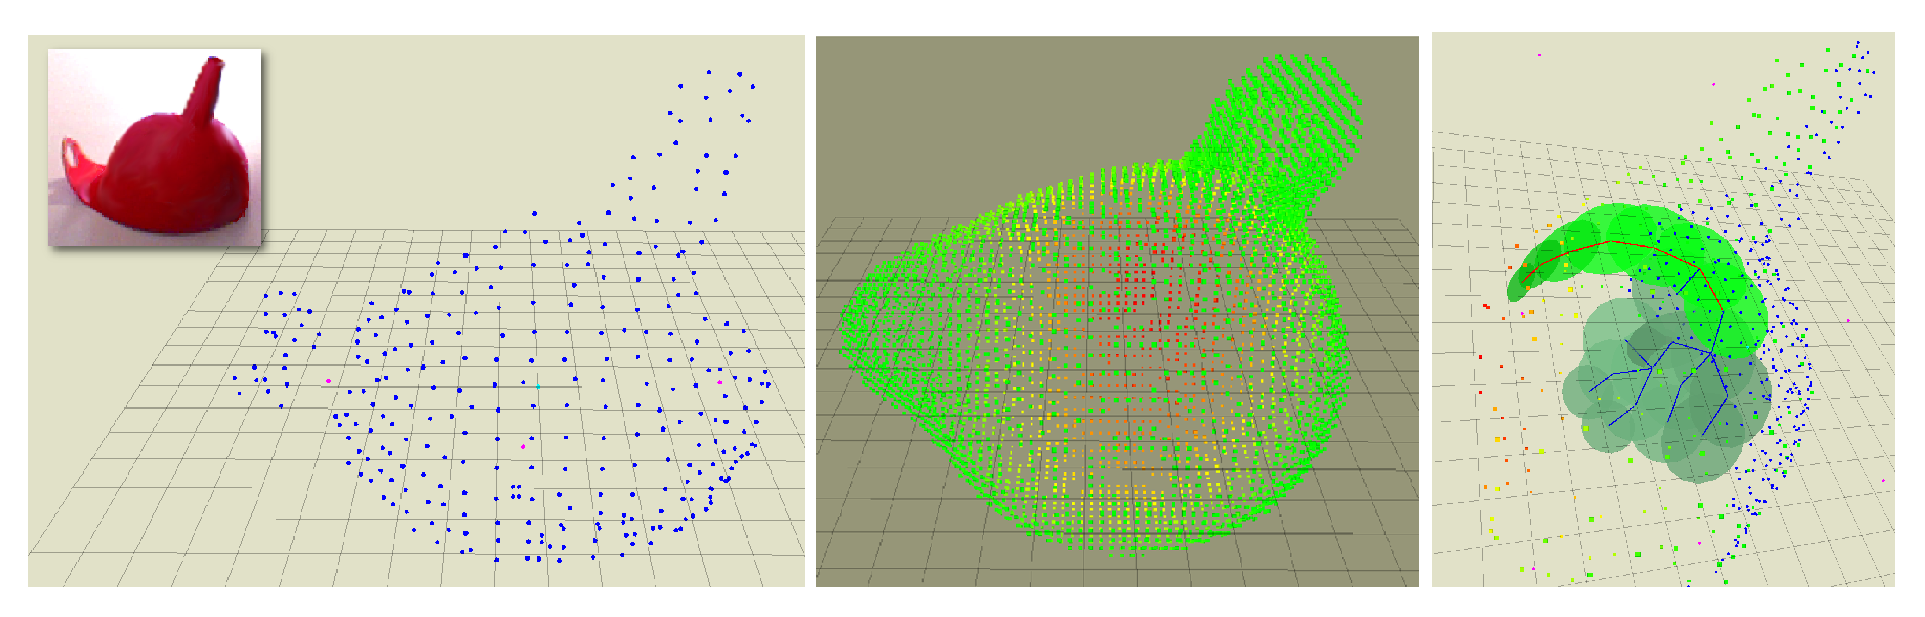
\includegraphics[width=0.95\linewidth]{funnel.eps}
    \caption{ A funnel (left-upper corner) is first seen by a depth camera. The segmented 3D points are shown in blue in the left figure to form the training set $\mathcal{S}^0$. The predicted shape by the GP on this set is shown in the middle obtained via a marching cube sampling algorithm. However, the GPAtlasRRT strategy does not require the explicit form of the predicted surface, as shown in the right figure. It works with the implicit form to devise the next-best tactile exploration shown in brighter green.}
    \label{fig:GPAtlasRRTfunnel}
\end{figure*}
Recall that this path lies on the predicted surface. Thus the controller to follow it must be compliant to avoid damage. The new tactile observations increase the training set, $\mathcal{S}^0$, reducing  the uncertainty of the surface model. Figures~\ref{fig:GPAtlasRRTtwo}~and~\ref{fig:GPAtlasRRTfunnel} show the Atlas RRT in the process of expansion on the implict surfaces for two partially explored objects. The next section describes how the GPAtlasRRT strategy is  embedded in a tactile exploration scenario.

\subsection{Tactile exploration using GPAtlasRRT}
\label{sec:gpatlasrrt_tactile_exploration}

The GPAtlasRRT algorithm is the planner that drives tactile exploration. This must be embedded in an overall execution and inference loop (Algorithm~\ref{alg:solution}). The initial, incomplete observation may be visual or tactile (lines to compute the model \ref{ini_gp}--\ref{fini_ini_gp}). Given this, the robot plans a sequence of touches, $\mathcal{P}$, (line \ref{exploration}), executes the next touch and updates the GP implicit surface model. We have now presented the inference and planning components. Now we present the execution component.

Several facts determine the difficulty of the problem and the shape of the solution for execution. First, to enable autonomous acquisition of near complete object models the robot should ideally be able to reorientate the object to expose different surfaces. This requires that the object be grasped by a second manipulator. Second, to minimise data errors due to object movement during exploration, the object must not move, so the grasp should be firm. However, a second feature of the problem is that the shape is not known. This makes obtaining a firm grasp challenging. We employed an underactuated manipulator (the Pisa/IIT
SoftHand~\cite{Catalano2014Adaptive}), which is both powerful and copes well with unmodelled contacts. 

There is then, however, a third problem. The view of the grasped object contains not only the object but also the hand. So the hand and object must be segmented from one another. Since underactuated hands do not typically possess position encoders, recovering the hand pose so as to segment the hand from the point cloud of the grasped object is non-trivial (line~\ref{segment_object}).

To tackle this we sensorized the SoftHand using IMUs~\cite{Santaera2015Lowcost} to recover the hand configuration. Using this information, together with the arm configuration, we crop the scene point cloud to separate the points on the object from those on the hand. The partial coverage of the object surface by the grasping hand limits the extent of the tactile exploration. This would require a re-grasp manoeuvre, which falls out of the scope of this paper.

\begin{algorithm}[t]
\textbf{\textsc{TactileExploration}}($\mathcal{Z}, \mathbb{V}_{\max})$\\ %functionname
\LinesNumbered
\DontPrintSemicolon
\SetAlgoVlined \SetKwInOut{Input}{input} \SetKwInOut{Output}{output}
\Input{An initial point cloud of the scene, $\mathcal{Z}$, and the desired variance, $\mathbb{V}_{\max}$, for the overall surface prediction.}
\Output{The object model as a Gaussian process, $\mathcal{GP}$.}
  \label{ini_gp} \If{ \textsc{isEmpty}($\mathcal{Z}$) }
  {
    $\mathcal{S}^0 \leftarrow $ \textsc{naiveProbe}() \\
  }
  \Else
  {
  \label{segment_object}  $\mathcal{S}^0 \leftarrow $ \textsc{segmentObject}($\mathcal{Z}$) \\
  }
  $\mathcal{S} \leftarrow$ \textsc{generateTrainSet}($\mathcal{S}^0$)
  $\mathcal{GP} \leftarrow $\textsc{computeModel}($\mathcal{S}$) \label{fini_ini_gp} \\
  \While { \texttt{true} } 
  {
    $\mathcal{P} \leftarrow $\textsc{GPAtlasRRT}($\mathcal{GP}, \mathbb{V}_{\max})$ \label{exploration} \\
    \If{ $\mathcal{P} \neq \varnothing$ }
    {
      \textsc{ApproachTo}($\mathcal{P}$, $\mathcal{GP}$) \label{approach} \\
      $\mathcal{S}^{0+} \leftarrow $\textsc{probeObject}($\mathcal{P}$) \label{probe} \\
      %$\mathcal{S}^0 \leftarrow$ \textsc{getOnSurface}($\tilde{\mathcal{S}^{0+}}$) \\
      %$\mathcal{S}^+ \leftarrow$ \textsc{getOutsideSurface}($\tilde{\mathcal{S}^{0+}}$) \\
      $\mathcal{S} \leftarrow$ \textsc{updateTrainSet($\mathcal{S}$, $\mathcal{S}^{0+}$)} \label{update_training} \\
      $\mathcal{GP} \leftarrow $\textsc{computeModel}($\mathcal{S}$) \label{re-compute} \\
      \textsc{MoveAway}($\mathcal{GP}$) \label{away} \\
    }
    \Else
    { 
      \Return {$\mathcal{GP}$} \label{solutionfound} \\
    }
  }
\caption{Surface modeling via GPAtlasRRT} \label{alg:solution}
\end{algorithm}

Having grasped the object, segmented it, inferred the initial GP model, and planned a sequence of touches, the robot finger moves to a pose from which it can initiate a movement to make the first touch (\textsc{approachTo}). This must be a safe distance from the predicted surface and normal to the target contact point. Since the object shape representation captures its uncertainty, a coarse point cloud is computed from the GP model and used to build a probabilistic collision map. Then, the robot moves to contact the surface\textsc{probeObject}, resulting in contact or non-contact. There are two schemes, in one the probe touches each point in the path $\mathcal{P}$. In the other only the final, high variance, point in $\mathcal{P}$ is touched.

The resulting position(s) $\mathbf{x}_i$ and target(s) $\mathbf{y}_i$ form a (series of) tuple(s) collected in the observation set $\mathcal{S}^{0+}$ (line \ref{probe}). During touch motions, collision avoidance is disabled and the probe moves compliantly. Once the end of the path is reached, the training set is updated (line \ref{update_training}). This is used to recompute a better model of the object surface, $\mathcal{GP}$ (line \ref{re-compute}). We then move the probe away (line \ref{away}). When the $\mathcal{GP}$ model has a maximum variance of $\mathbb{V}_{\max}$ for any point on the implicit surface, that is, $\mathbb{V}[f(\mathbf{x})] < \mathbb{V}_{\max}, \, \forall \mathbf{x} \in \mathcal{X}$, exploration terminates.

The next section presents two experimental studies, one in simulation, where \textsc{probeObject} is performed by ray-casting on object meshes, and a real robot experiment.

% During the \textsc{ApproachTo} (line~\ref{approach}) (\textsc{MoveAway}, line~\ref{away}) phases, the robot uses position control and standard motion planning techniques with collision avoidance. Since we are modelling the shape, we need to ensure that everytime the robot moves close (away) from the object, it does not collide with the object. It is tentative to use the current estimated shape, but since we are not actually computing it explicitly in our approach, we choose the bounding sphere as the collision geometry of the object. Thus the robot moves towards (away from) the surface at the contact location in the normal direction until reaching the bounding sphere. After that, a standard motion planning is used to approach the object (get to the rest position).

% The \textsc{probeObject} (line~\ref{probe}) phase is engaged once the robot is within the bounding sphere. The robot uses Cartesian impedance control, with the Cartesian force, pose and impedance set properly for the given setup. These implementation details are given in the next section. Since we don't actually know where the surface is, we need to whether the robot actually touched something or not, in order to properly label the acquisition (lines~\ref{belonglabel} and~\ref{nobelonglabel}) 

% The method finishes when \textsc{exploreGPAtlasRRT} (line~\ref{exploration}) described in Algorithm~\ref{algo:strategy} has explore sufficiently the estimated shape and could not find an exploratory action $\Gamma$ (line~\ref{solutionfound}), i.e. the object shape is probabilistically estimated within the 95\% of the confidence interval computed from $\mathbb{V}_{des}$. 

%The complete solution of the problem as stated in~\ref{sec:scope} is depicted in Algorithm~\ref{alg:solution}.



%This section provides a more detailed description of our GPAtlasRRT algorithm. As described in Sec.~\ref{sec:scope}, our approach combines probabilistic inference on an unknown surface with a asymptotically optimal sample-based exploration technique for implicitly-defined configuration spaces (manifolds). We demonstrate the efficiency of our proposed solution in a bimanual framework (see Sec.~\ref{sec:scenario}) where a humanoid robot (Vito) can hold an unknown object in one hand and actively build up a probabilistic model of the object's shape by integrating visual and haptic information. This is done efficiently by selecting haptic actions which lead to an asymptotically optimal reduction of the global shape uncertainty of the model. 

%We employ a GP to learn a probabilistic model of the object surface, encoded as an implicit surface, constrained to visual and tactile clues iteratively acquired. First we rely on visual information captured by a RGB-D camera, which will be pre-processed, as described in Sec.~\ref{sec:segmentation}, to isolate the object's point cloud from the rest of the scene (robot's and environment's). Secondly we generate artificial points to improve the performance of the GP estimation, and after having labelled them properly we pass them as training inputs to the GP procedure. This procedure will be described in Sec.~\ref{sec:shape}. 

% The (noisy) visual observations constrain our model which has the effect of increasing its confidence (reduced variance) on its predictions about the function value $f(\mathbf{x})$ in regions highly populated by the training dataset. However, predictions in occluded or unseen regions will be associated with lower confidence (high uncertainty) since few or none information are available.  

% To improve the accuracy of our model, we make inference on it to build paths along the estimated object's surface such that a robot finger equipped with F/T sensors can collect haptic information over unseen regions of the surface. Since the surface is encoded as an implicit surface we need a more efficient way to make inference than to just attempt to reconstruct the expected object's shape via a highly-dense randomly generated samples. Instead we utilise the notion of manifold as a collection of local parametrisation (charts) such that we can make predictions on the neighbouring regions of already visited points as well as generate more charts on the more recent visited regions. To keep track of how the charts are generated and connected by themselves, we employ an RRT-like algorithm to build a tree of charts. The algorithm terminates when a path to a region, which is more promising to reduce the overall shape uncertainty of our model, is found.

%Section~\ref{sec:strategy} will explain the novelty of our algorithm in detail.  


% \begin{algorithm}[h]
% \textbf{\textsc{createGaussianProcess}}($X$)\\ %functionname
% \LinesNumbered
% \DontPrintSemicolon
% \SetAlgoVlined \SetKwInOut{Input}{input} \SetKwInOut{Output}{output}
% \Input{The training data, $\mathcal{X}$, in the form of a point cloud.}
% \Output{The Gaussian Process that models the object shape.}
%   $\mathcal{D} \leftarrow$\textsc{deMeanNormalizeAndLabel}(\{$\mathcal{X}$, $\mathbf{0}_{\text{sizeOf}(\mathcal{X})}$\}) \\
%   \textsc{addLabeledPoint}(\{$\mathbf{0}_3, -1\}$, $\mathcal{D}$) \\
%   \textsc{addLabeledPoints}(\{\textsc{sphere}$(\mathbf{0}_3, 1.1, N)$, $+\mathbf{1}_{N}\}$, $\mathcal{D}$) \\
%   $\mathcal{G} \leftarrow$ \textsc{doRegression}($\mathcal{D}$) \\
%   \Return $\mathcal{G}$ \\
% \caption{Gaussian Process regression} \label{algo:strategy}
% \end{algorithm}

%%%%%%%%%%%%%%%%%%%%%%%%%%%%%%%%%%%%%%%%
%\subsection{Best-next tactile strategy}
%\label{sec:strategy}

%Algorithm~\ref{alg:strategy} presents a pseudo-code of our implementation. As previously described in Sec.~\ref{sec:scope}, we explore the estimated surface of the object via a combination of probabilistic inference and sample-based techniques for manifolds. 

%We employ an RRT-like algorithm which, instead of growing in the ambient space, is embedded in an implicitly defined configuration space defined by a manifold or Atlas, $\mathcal{A}$. The major difference between our proposed implementation and a traditional RRT-algorithm is in how we select a new candidate node and expand the tree.


%
%The RRT explorer, however does not have any information on the model on which is built, specifically,
%it just need to track the connections between nodes of the tree and decide where it
%should expand next. All the model information is stored in an Atlas, called $\mathcal{A}$.
%
%An atlas can be viewed as a collection of maps or charts and conceptually it is able
%to create new charts at a given location on the surface it is currently modelling.
%Furthermore $\mathcal{A}$ is able to expand a given chart, producing new locations
%from where create new charts.
%
%In the proposed exploration strategy, RRT nodes are exactly the charts, thus
%building such a tree is like composing an atlas, which tries to model the implicit
%estimated surface.
%
%Formally we define a chart $\mathcal{C}$ with a center point on the surface $\mathbf{x}_{c}$,
%such that
%$$
%\mathbb{E}(\mathcal{S}(\mathbf{x}_c)) \approx 0
%$$
%with a search space defined as a
%tangent disc at the surface, centered on $\mathbf{x}_c$, with radius 
%$$
%R \propto \frac{1}{\mathbb{V}(\mathcal{S}(\mathbf{x}_c))}
%$$ 
%and finally with the gradient information at the center 
%$$
%G \approx \frac{\partial \mathcal{S}}{\partial \mathbf{x}}
%$$
%Conventionally the center variance is addressed as the chart variance, because
%it locally approximates the uncertainty of the surface estimation.
%
%With such charts, the atlas can be defined as the set of all charts plus some parameters
%responsible for chart creation:
%$$
%\mathcal{A} \triangleq \{\mathcal{C}_1, \ldots, \mathcal{C}_i, \ldots, \mathcal{C}_n, \Omega^{\mathcal{A}}\}
%$$
%where $n$ is the number of created charts and $\Omega^{\mathcal{A}}$ are the parameters.
%
%The explorer can also be viewed as a collection of chart connections, or branches,
%plus another set of parameters responsible for the tree expansion behaviour:
%$$
%\mathcal{T} \triangleq \{\mathcal{C}_i \leftarrow \mathcal{C}_j, \ldots, \Omega^{\mathcal{T}}\}_{i \neq j \le n}
%$$



%Given a Gaussian Process model, $\mathcal{M}$, approximating the implicit object surface
%with a regression, as described in Sec.~\ref{sec:gpr}, and the set of parameters
%$$\Omega \triangleq \Omega^{\mathcal{A}} \cup \Omega^{\mathcal{T}}$$
%An empty atlas and a RRT explorer can be initialized.
%Then a starting point is selected randomly among the object training set:
%$$
%\mathbf{x}_{c,i} \in \chi^0
%$$
%where $\chi^0$ is the set of object points,
%which in turn is part of the Gaussian Process Model, $\mathcal{M}$.
%
%$\mathcal{A}$ is charged to create the first chart, also called \emph{root}, from the starting point,
%then the algorithm rapidly builds the tree of charts on the object until the supplied termination
%criterion is met, or the maximum allowed number of charts has been reached.
%The best-next tactile action is finally the path from the converging chart to the root, or nothing if no such chart exists.

%The main loop of the algorithm is fulfilled by the following steps:\\
%\begin{inparadesc}
%\item[select($\cdot$)] Ask the explorer to select a chart to expand,
%among the chart collection ($\mathcal{A}$).
%This is done by selecting one at random with a bias to increase the probability
%of selecting the last created chart. This criterion is adopted to grow a tree
%which is more inclined to expand on a single branch, but at the same time maintain the
%possibility to create new branches from previous charts. So efficiency and speed
%is preserved, while we make sure we are exploring as much surface as possible,
%before reaching a solution.\\
%\item[expand($\cdot$)] The selected chart $\mathcal{C}_j$ is expanded by $\mathcal{A}$, by
%sampling $k$ points on its tangent discs then selecting one at maximum variance
%and at the same time not in collision with other charts search spaces. 
%So a sample $\mathbf{s}_i$ is selected if 
%$$
%\mathit{max}_{i\in k}[\mathbb{V}(\mathcal{S}(\mathbf{s}_i))]
%$$
%and 
%$$
%{\parallel\mathbf{s}_i - \mathbf{x}_{c,j}\parallel}_{2} > R_j, \forall \mathcal{C}_j \in \mathcal{A}_{i \ne j}
%$$
%where $\mathbf{x}_{c,j}$ is the center and $R_j$ is the tangent disc radius of $\mathcal{C}_j$.

%The selected $\mathbf{s}_i$ is then projected back on the surface,
%creating a center for a new chart, $\mathbf{x}_{c,k}$.
%The projection is performed with a gradient descend method, using the gradient estimation
%of the chart $G_j$.\\
%\item[create($\cdot$)] A new chart  is created on the projected point, maintaining the atlas
%    expansion on the estimated implicit surface
%$$
%\mathcal{C}_k \in \mathcal{A}
%$$
%\item[connect($\cdot$)] creates a connection to the chart which originated the newly created one,
%    drawing a new branch for the tree
%$$
%\{\mathcal{C}_j \leftarrow \mathcal{C}_k \} \in \mathcal{T}
%$$
%\end{inparadesc}

%$\mathcal{C}_k$ is then tested for the termination condition and the whole loop
%starts anew.

%The progressively growing tree of charts expands on the object surface until
%the termination criterion is met. Then, when this happens, the procedure terminates and the full
%path from the converging chart to the root of the tree is reported as a solution.

%Furthermore, to customize the exploration, the parameters in $\Omega^{\mathcal{A}}$ 
%control how much chart search spaces are big according to their variances and how many
%samples are generated during the \textsc{expand}($\cdot$) phase. 
%We chose to create tangent disc radii inversely proportional to their variance,
%because, when the uncertainty/variance is low, we want to expand further
%away from the starting chart, traversing reasonably certain surfaces faster.
%On the contrary, when the uncertainty/variance is high, we want to make small
%exploration steps, because we are not certain of the underlaying estimated surface.

%We chose to have a variance threshold as a termination condition, defined in $\Omega^{\mathcal{T}}$,
%because when the exploration reaches a chart with high variance, we want to stop
%the exploration and perform a tactile action there to reduce the uncertainty in the
%model. 
%% The action will bring new data to update the shape estimation and eventually 
% a new more accurate exploration can be started with updated model.
